%% ============================================================
%%  ECGenius — IEEE Journal Manuscript
%%  "Ontology-Guided Differential Diagnosis for Explainable
%%   ECG Interpretation Using Rule-Based and Bayesian Clinical
%%   Reasoning"
%%
%%  Authors: Yash Ghule, Dr. Annushree Bablani
%%  IIIT Sri City, Andhra Pradesh, India
%%
%%  Compile with: pdflatex → bibtex → pdflatex → pdflatex
%%  (or: latexmk -pdf ecgenius_ieee.tex)
%% ============================================================
\documentclass[journal]{IEEEtran}

%% ---- Packages -----------------------------------------------
\usepackage{amsmath,amssymb,amsfonts}
\usepackage{algorithmic}
\usepackage{algorithm}
\usepackage{array}
\usepackage{textcomp}
\usepackage{booktabs}
\usepackage{multirow}
\usepackage{graphicx}
\usepackage{xcolor}
\usepackage{url}
\usepackage{cite}
\usepackage{balance}
\usepackage{enumitem}

%% ---- TikZ ---------------------------------------------------
\usepackage{tikz}
\usetikzlibrary{%
  shapes.geometric,
  shapes.misc,
  arrows.meta,
  positioning,
  fit,
  calc,
  backgrounds,
  decorations.pathreplacing,
  matrix}

%% ---- TikZ style definitions ---------------------------------
\tikzset{
  %% General flow boxes
  flowbox/.style={
    rectangle, rounded corners=3pt,
    draw=black!60, fill=blue!7,
    text width=1.95cm, align=center,
    minimum height=0.70cm, font=\scriptsize\sffamily},
  %% Critical / Tier-1 boxes
  critbox/.style={
    rectangle, rounded corners=3pt,
    draw=red!70, fill=red!8,
    text width=1.95cm, align=center,
    minimum height=0.70cm, font=\scriptsize\sffamily\bfseries},
  %% NB / Bayesian boxes
  nbbox/.style={
    rectangle, rounded corners=3pt,
    draw=purple!60, fill=purple!7,
    text width=2.20cm, align=center,
    minimum height=0.70cm, font=\scriptsize\sffamily},
  %% Ontology hierarchy nodes
  rootnode/.style={
    ellipse, draw=black!70, fill=gray!15,
    align=center, font=\scriptsize\bfseries,
    minimum width=1.2cm, minimum height=0.55cm},
  catnode/.style={
    rectangle, rounded corners=2pt,
    draw=blue!60, fill=blue!10,
    align=center, font=\scriptsize,
    minimum width=1.5cm, minimum height=0.50cm},
  leafnode/.style={
    rectangle, draw=green!60!black, fill=green!7,
    align=center, font=\tiny,
    minimum width=1.2cm, minimum height=0.45cm},
  patnode/.style={
    rectangle, draw=orange!70, fill=orange!8,
    align=center, font=\tiny,
    minimum width=1.2cm, minimum height=0.45cm},
  %% Decision diamond
  decision/.style={
    diamond, aspect=2.2,
    draw=orange!70, fill=orange!10,
    text width=1.6cm, align=center,
    font=\scriptsize\sffamily,
    inner sep=0pt},
  %% Arrows
  arrow/.style={-{Stealth[scale=1.1]}, thick, black!70},
  darrow/.style={-{Stealth[scale=0.9]}, thick, dashed, gray!70},
  rarrow/.style={-{Stealth[scale=1.0]}, thick, red!70},
}

%% ---- Hyperref (load last) -----------------------------------
\usepackage{hyperref}
\hypersetup{colorlinks=true, linkcolor=blue!60!black,
            citecolor=blue!60!black, urlcolor=blue!60!black}

%% ============================================================
\begin{document}

\title{Ontology-Guided Differential Diagnosis for Explainable ECG
Interpretation Using Rule-Based and Bayesian Clinical Reasoning}

\author{Yash~Ghule,~\IEEEmembership{Student Member,~IEEE,}
        and~Dr.~Annushree~Bablani,~\IEEEmembership{Member,~IEEE}
\thanks{Both authors are with the Department of Electronics and
Communication Engineering, Indian Institute of Information Technology
Sri City, Chittoor District, Andhra Pradesh 517646, India
(e-mail: ecgenius.life@gmail.com).}
\thanks{Manuscript received \today.}
}

\markboth{IEEE Journal of Biomedical and Health Informatics,~Vol.~XX,
No.~XX, XXXX}{%
Ghule \MakeLowercase{\textit{et al.}}: Ontology-Guided Differential
Diagnosis for Explainable ECG Interpretation}

\maketitle

%% ---- Abstract -----------------------------------------------
\begin{abstract}
Automated interpretation of 12-lead electrocardiograms (ECGs) remains
a challenging problem due to the complexity of cardiac electrophysiology,
the rarity of life-threatening arrhythmias, and the clinical imperative
of zero missed critical diagnoses.
Existing deep-learning approaches yield high aggregate accuracy but
suffer from opacity, lack of structured clinical knowledge, and
inadequate safety guarantees for time-sensitive conditions.
We present \textit{ECGenius}, an ontology-guided clinical decision
support system (CDSS) that integrates a lightweight multi-scale
convolutional neural network (LightV2, ${\approx}362$K parameters)
with a structured clinical ontology, a cardiologist-rule engine, and
a Naive Bayesian decision fusion module.
The ontology comprises 35 nodes organized across five cardiac
categories—Rhythm, Ischemia, Structural, Conduction, and ECG
Pattern—and provides SNOMED-CT, ICD-10, and AHA guideline mappings
for every diagnostic label.
The rule engine encodes four categories of clinical constraints,
including derived-diagnosis injection for rare but critical patterns
(Sgarbossa criteria for LBBB-associated STEMI, Wellens syndrome
T-wave inversion, and Torsades de Pointes risk).
Decision fusion combines ECG-derived prior probabilities with
patient history evidence through 98 conditional probability table
entries in numerically stable log-space, with a hard safety override
ensuring that life-threatening diagnoses are never suppressed
regardless of posterior magnitude.
A multi-layer explainability framework generates per-diagnosis audit
trails, likelihood-ratio narratives, and score decompositions suitable
for clinical review and regulatory audit.
Full experimental validation on the AIIMS Nagpur and PhysioNet
CinC\,2020/2021 cohorts is ongoing; this manuscript presents the
complete system architecture, methodology, and experimental design
with clearly marked placeholders for prospective results.
\end{abstract}

\begin{IEEEkeywords}
12-lead ECG, clinical decision support, differential diagnosis,
ontology, Naive Bayes fusion, explainable AI, rule-based reasoning,
Sgarbossa criteria, Wellens syndrome, convolutional neural network,
temporal convolutional network.
\end{IEEEkeywords}

%% ============================================================
\section{Introduction}
\label{sec:intro}

\IEEEPARstart{T}{he} 12-lead electrocardiogram is among the most
frequently ordered diagnostic tests in medicine, with over
300 million recordings performed annually worldwide
\cite{hannun2019cardiologist}.
Accurate and timely ECG interpretation is essential for diagnosing
life-threatening conditions such as ST-elevation myocardial infarction
(STEMI), ventricular fibrillation (VF), and complete atrioventricular
block, where treatment delays are directly correlated with mortality.
However, ECG interpretation demands substantial expertise, and
inter-reader variability remains clinically significant even among
trained cardiologists \cite{ribeiro2020automatic}.

Recent advances in deep learning have produced models that match or
exceed cardiologist-level accuracy on certain arrhythmia detection
tasks \cite{hannun2019cardiologist,ribeiro2020automatic,
strodthoff2020deep}.
These systems, however, share three structural limitations.
First, they produce \emph{point predictions} without differential
diagnosis ranking, clinical evidence traceability, or structured
triage classifications.
Second, they lack mechanisms for encoding explicit cardiologist
knowledge such as Sgarbossa criteria for LBBB-associated STEMI
\cite{sgarbossa1996electrocardiographic} or Wellens syndrome
\cite{zwaan1989wellens}, which are rare but clinically critical
patterns that require specialist recognition.
Third, they are not designed with hard safety constraints: a
life-threatening prediction at low posterior probability can be
silently suppressed by a competing, higher-confidence benign
prediction.

Ontology-based clinical decision support systems (CDSS) have a long
history in medicine \cite{shortliffe2001biomedical}, providing
structured knowledge representation, hierarchical reasoning, and
interoperability with standard terminologies such as SNOMED-CT
\cite{snomedct} and ICD-10 \cite{icd10}.
Bayesian reasoning frameworks offer a principled mechanism for
combining heterogeneous evidence sources—ECG features, patient
symptoms, risk factors, and vital signs—into calibrated posterior
probabilities \cite{spiegelhalter1986probabilistic}.
The integration of these complementary paradigms with modern
deep-learning models creates an opportunity for CDSS that is
simultaneously accurate, interpretable, and clinically safe.

This paper presents \textbf{ECGenius}, an ontology-guided differential
diagnosis system for 12-lead ECG interpretation.
The system is designed around four guiding clinical principles:
(i) \emph{never suppress a critical diagnosis}—hard safety overrides
ensure that Tier-1 life-threatening conditions are always surfaced;
(ii) \emph{transparency by design}—every ranked output carries a
full evidence trail and score decomposition;
(iii) \emph{knowledge augmentation}—a data-driven rule engine injects
diagnoses implied by cardiologist knowledge but below the model's
detection threshold; and
(iv) \emph{standard interoperability}—all labels carry SNOMED-CT,
ICD-10, and AHA guideline identifiers.

\subsection*{Summary of Contributions}

\begin{enumerate}
  \item \textbf{Clinical Ontology for ECG.}
        A 35-node hierarchical ontology spanning five cardiac
        categories with three-tier triage classification and
        standard medical terminology mappings.

  \item \textbf{Data-Driven Clinical Rule Engine.}
        A CSV-driven, handler-registered rule engine supporting
        mutual exclusion, precedence, derived-diagnosis injection,
        and downgrade rules, including explicit encoding of
        Sgarbossa criteria, Wellens patterns, and Torsades de
        Pointes risk.

  \item \textbf{Naive Bayesian Decision Fusion in Log-Space.}
        A numerically stable multi-class Naive Bayes fusion module
        combining ECG-derived prior probabilities with patient
        history through 98 conditional probability table entries,
        with a hard Tier-1 safety override.

  \item \textbf{Multi-Layer Explainability Framework.}
        Per-diagnosis audit trails, likelihood-ratio narratives,
        score decompositions, and clinical action recommendations
        derived entirely from structured internal state, without
        post-hoc approximation.
\end{enumerate}

The remainder of this paper is organized as follows.
Section~\ref{sec:related} reviews related work.
Sections~\ref{sec:arch}--\ref{sec:model} describe the system
architecture and neural network model.
Sections~\ref{sec:ontology}--\ref{sec:explainability} detail the
clinical reasoning layers.
Sections~\ref{sec:impl}--\ref{sec:results} cover implementation,
experimental design, and results.
Sections~\ref{sec:discussion}--\ref{sec:conclusion} discuss findings,
limitations, future work, and conclusions.

%% ============================================================
\section{Related Work}
\label{sec:related}

\subsection{Deep Learning for ECG Interpretation}

The application of deep neural networks to ECG analysis has
progressed rapidly since the landmark study of Hannun
\textit{et al.} \cite{hannun2019cardiologist}, which demonstrated
cardiologist-level arrhythmia detection from single-lead ambulatory
recordings.
Ribeiro \textit{et al.} \cite{ribeiro2020automatic} extended this
to 12-lead ECGs using a residual neural network trained on over
2 million records, showing superior performance on six ECG conditions.
The PhysioNet/Computing in Cardiology Challenges 2020 and 2021
\cite{reyna2020physionet,reyna2021physionet} established multi-label
classification benchmarks across diverse ECG datasets, spurring
numerous architectures including attention-enhanced
residual networks, LSTM-CNNs, and transformer-based models.
Strodthoff \textit{et al.} \cite{strodthoff2020deep} conducted a
systematic benchmark on the PTB-XL dataset \cite{wagner2020ptb},
demonstrating that temporal convolutional networks (TCN)
\cite{bai2018empirical} with appropriate depth and dilation achieve
competitive performance with significantly fewer parameters than
recurrent alternatives.
Squeeze-and-Excitation (SE) attention \cite{hu2018squeeze} has
been shown to improve multi-label ECG classification by adaptively
recalibrating channel feature responses.

Despite high aggregate accuracy, these systems do not generate
differential diagnoses, do not incorporate patient clinical context,
and provide limited explainability beyond attention weight
visualization.

\subsection{Clinical Ontologies and Knowledge-Based CDSS}

Ontology-based clinical decision support has a rich history in
biomedical informatics \cite{shortliffe2001biomedical}.
The SNOMED-CT terminology \cite{snomedct} provides over 350,000
clinical concepts with formal subsumption relationships, enabling
interoperable clinical reasoning.
Clinical applications of ontological reasoning have been reported in
radiology, pathology, and cardiology, with systems such as
INTERNIST-1 and QMR demonstrating the value of structured clinical
knowledge for differential diagnosis generation
\cite{miller1982internist}.
More recently, ontology-driven approaches have been applied to
integrate ECG features with clinical guidelines for structured
reporting \cite{beinlich2018ecg}.
However, most existing ECG CDSS systems either use flat label
classifications without hierarchical reasoning or apply hard-coded
rule libraries without data-driven weight calibration.

\subsection{Bayesian Reasoning in Clinical Decision Support}

Probabilistic reasoning has long been central to medical diagnosis.
Spiegelhalter and Knill-Jones \cite{spiegelhalter1986probabilistic}
demonstrated the utility of Naive Bayes classifiers for clinical
differential diagnosis, showing strong performance despite the
conditional independence assumption.
More recent work on Bayesian networks for clinical decision support
\cite{lucas2004bayesian} has shown that even simple models can
outperform experienced clinicians on specific diagnostic tasks when
prior probabilities and likelihoods are well-calibrated.
The likelihood ratio framework \cite{deeks2004likelihood} provides
an intuitive basis for evidence-weighted reasoning and remains
widely used in evidence-based medicine.
For ECG interpretation specifically, Bayesian approaches have been
applied to the diagnosis of acute myocardial infarction
\cite{kennedy1996bayesian}, demonstrating the complementarity of
electrocardiographic features and clinical history.

\subsection{Explainability in Medical Artificial Intelligence}

The clinical deployment of AI systems necessitates explanation
mechanisms that are meaningful to clinicians \cite{caruana2015intelligible}.
Post-hoc approximation methods such as LIME \cite{ribeiro2016lime}
and SHAP \cite{lundberg2017unified} have been applied to ECG
classifiers to generate input-attribution explanations, but these
do not produce differential diagnoses or structured clinical reasoning
chains.
For CDSS, explanation by construction—deriving explanations directly
from the system's internal reasoning structure—is preferable to
post-hoc approximation, as it guarantees consistency and
auditability \cite{shortliffe2001biomedical}.
Our system adopts explanation-by-construction as a core design
principle, deriving all explanations from structured internal state.

%% ============================================================
\section{System Architecture}
\label{sec:arch}

ECGenius is a five-stage pipeline that transforms a raw 12-lead ECG
signal into a ranked differential diagnosis list with evidence-weighted
confidence scores, clinical triage recommendations, and per-diagnosis
audit trails.
Fig.~\ref{fig:pipeline} illustrates the complete architecture.

The stages are:
\begin{enumerate}[leftmargin=*]
  \item \textbf{Signal Preprocessing.} Bandpass filtering, notch
        filtering, resampling, segmentation, and per-lead
        z-score normalization.
  \item \textbf{Neural Network Inference.} LightV2, a multi-scale
        1D TCN, produces multi-label sigmoid probabilities for 15
        ECG conditions.
  \item \textbf{Ontology Mapping.} Model outputs are enriched with
        hierarchical labels, triage tiers, SNOMED-CT/ICD-10 codes,
        and mutual exclusion rules are applied.
  \item \textbf{Clinical Rule Engine.} Cardiologist-defined rules
        enforce precedence constraints and inject derived diagnoses
        implied by pattern-trigger combinations.
  \item \textbf{Bayesian Decision Fusion.} Patient history evidence
        is combined with ECG-derived priors via Naive Bayes fusion,
        yielding ranked posteriors with confidence labels and safety
        overrides.
\end{enumerate}

An \textbf{explainability layer} operates across stages 3–5,
accumulating a per-diagnosis audit trail, likelihood-ratio evidence
breakdowns, and a clinician-facing narrative.

\begin{figure*}[!t]
\centering
%% ---- Figure 1: ECGenius Pipeline ----
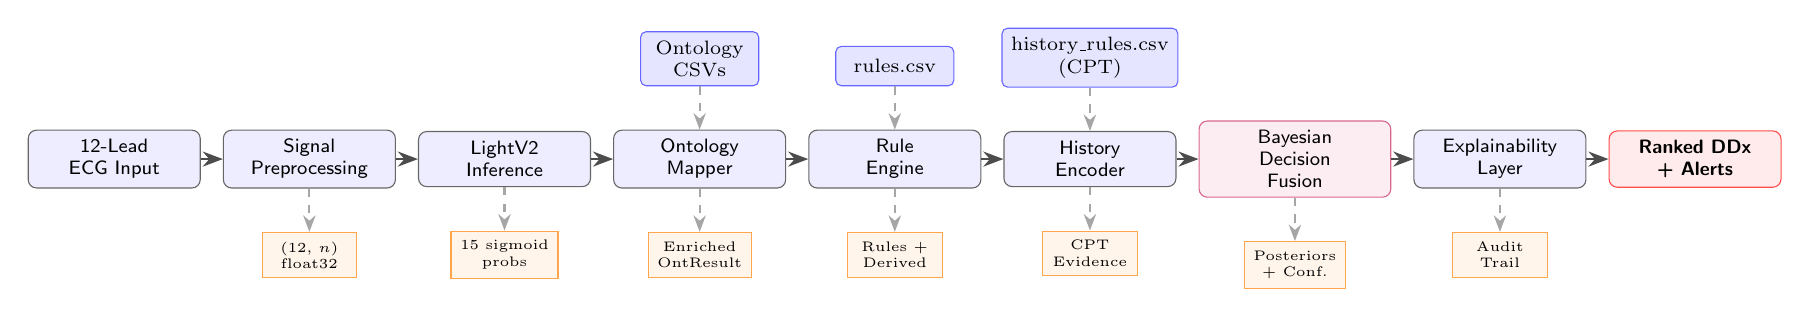
\begin{tikzpicture}[node distance=0.35cm and 0.28cm]

  %% Row 1: main pipeline
  \node[flowbox] (ecg)   {12-Lead\\ ECG Input};
  \node[flowbox, right=of ecg]  (prep)  {Signal\\ Preprocessing};
  \node[flowbox, right=of prep] (model) {LightV2\\ Inference};
  \node[flowbox, right=of model](onto)  {Ontology\\ Mapper};
  \node[flowbox, right=of onto] (rules) {Rule\\ Engine};
  \node[flowbox, right=of rules](hist)  {History\\ Encoder};
  \node[nbbox,   right=of hist] (fuse)  {Bayesian\\ Decision\\ Fusion};
  \node[flowbox, right=of fuse] (xai)   {Explainability\\ Layer};
  \node[critbox, right=of xai]  (out)   {Ranked DDx\\ + Alerts};

  %% Main arrows
  \draw[arrow] (ecg)   -- (prep);
  \draw[arrow] (prep)  -- (model);
  \draw[arrow] (model) -- (onto);
  \draw[arrow] (onto)  -- (rules);
  \draw[arrow] (rules) -- (hist);
  \draw[arrow] (hist)  -- (fuse);
  \draw[arrow] (fuse)  -- (xai);
  \draw[arrow] (xai)   -- (out);

  %% Row 2: data artifacts below
  \node[patnode, below=0.55cm of prep]  (raw)  {(12, $n$)\\ float32};
  \node[patnode, below=0.55cm of model] (prob) {15 sigmoid\\ probs};
  \node[patnode, below=0.55cm of onto]  (enr)  {Enriched\\ OntResult};
  \node[patnode, below=0.55cm of rules] (mut)  {Rules +\\ Derived};
  \node[patnode, below=0.55cm of hist]  (hd)   {CPT\\ Evidence};
  \node[patnode, below=0.55cm of fuse]  (post) {Posteriors\\ + Conf.};
  \node[patnode, below=0.55cm of xai]   (nar)  {Audit\\ Trail};

  \draw[darrow] (prep)  -- (raw);
  \draw[darrow] (model) -- (prob);
  \draw[darrow] (onto)  -- (enr);
  \draw[darrow] (rules) -- (mut);
  \draw[darrow] (hist)  -- (hd);
  \draw[darrow] (fuse)  -- (post);
  \draw[darrow] (xai)   -- (nar);

  %% External data sources
  \node[catnode, above=0.55cm of onto,  xshift=0.0cm] (ontcsv){Ontology\\ CSVs};
  \node[catnode, above=0.55cm of rules, xshift=0.0cm] (rcsv)  {rules.csv};
  \node[catnode, above=0.55cm of hist,  xshift=0.0cm] (hcsv)  {history\_rules.csv\\ (CPT)};

  \draw[darrow] (ontcsv) -- (onto);
  \draw[darrow] (rcsv)   -- (rules);
  \draw[darrow] (hcsv)   -- (hist);

\end{tikzpicture}
\caption{ECGenius end-to-end pipeline. Top row: processing stages.
Middle row: data artifacts at each stage boundary.
Bottom dashed arrows: external knowledge sources loaded at startup.
The \textit{orange} nodes indicate ECG pattern triggers used as
rule inputs but excluded from the final DDx list.
The \textit{purple} Bayesian Fusion node is the primary scoring engine.}
\label{fig:pipeline}
\end{figure*}

%% ============================================================
\section{ECG Signal Preprocessing}
\label{sec:preprocess}

Raw ECG signals are accepted in WFDB MATLAB format (PhysioNet
\texttt{.mat}) or comma-separated format (\texttt{.csv}).
The preprocessing pipeline (Algorithm~\ref{alg:preprocess}) converts
any valid input into a standardized $(\textit{12},\ 5000)$
float32 tensor at 500\,Hz.

\begin{algorithm}[t]
\caption{ECG Preprocessing Pipeline}
\label{alg:preprocess}
\begin{algorithmic}[1]
  \REQUIRE Raw ECG $\mathbf{X} \in \mathbb{R}^{N_\ell \times N_t}$,
           source sampling rate $f_s$
  \ENSURE  Preprocessed ECG $\hat{\mathbf{X}} \in \mathbb{R}^{12 \times 5000}$
  \STATE   \textbf{Reshape:} detect and transpose if $(N_t, 12)$;
           replicate if single-lead; truncate if $N_\ell > 12$
  \STATE   \textbf{Bandpass:} Butterworth order-4, $[0.5,\ 40]$~Hz
           via zero-phase \texttt{filtfilt}
  \STATE   \textbf{Notch:} IIR notch filter at $f_{notch}=50$~Hz,
           quality factor $Q=30$, via zero-phase \texttt{filtfilt}
  \STATE   \textbf{Resample:} \texttt{scipy.signal.resample} to
           $f_{target}=500$~Hz
  \STATE   \textbf{Segment:} extract center 5000-sample window;
           edge-pad if $N_t < 5000$
  \STATE   \textbf{Normalise:} per-lead z-score:
           $\hat{x}_\ell = (x_\ell - \mu_\ell)
           / \max(\sigma_\ell,\ 10^{-8})$
  \STATE   \textbf{Quality check:} flag flat leads
           ($\text{range} < 0.01$) and noisy leads
           ($\text{range} > 10.0$)
  \RETURN  $\hat{\mathbf{X}}$ (shape $12 \times 5000$, float32)
\end{algorithmic}
\end{algorithm}

Zero-phase filtering via \texttt{filtfilt} is used throughout to
eliminate phase distortion that would otherwise shift the temporal
relationships between fiducial points (P-wave onset, QRS complex,
T-wave peak) critical for interval measurement.
The center-window segmentation strategy is preferred over
leading-edge cropping to avoid lead-connection artifacts that
are typically concentrated in the first 500–1000 samples.
Edge padding is applied when the recording is shorter than 10\,s,
as it preserves signal statistics better than zero-padding for
ECG data, which has non-zero local baselines.

%% ============================================================
\section{Neural Network Architecture: LightV2}
\label{sec:model}

LightV2 (LightECGNet version 2) is a multi-label 1D convolutional
classifier designed for efficiency and clinical deployment.
The complete architecture is illustrated in Fig.~\ref{fig:model_arch}
and described in Sections~\ref{sec:model}A--D below.

\begin{figure}[!t]
\centering
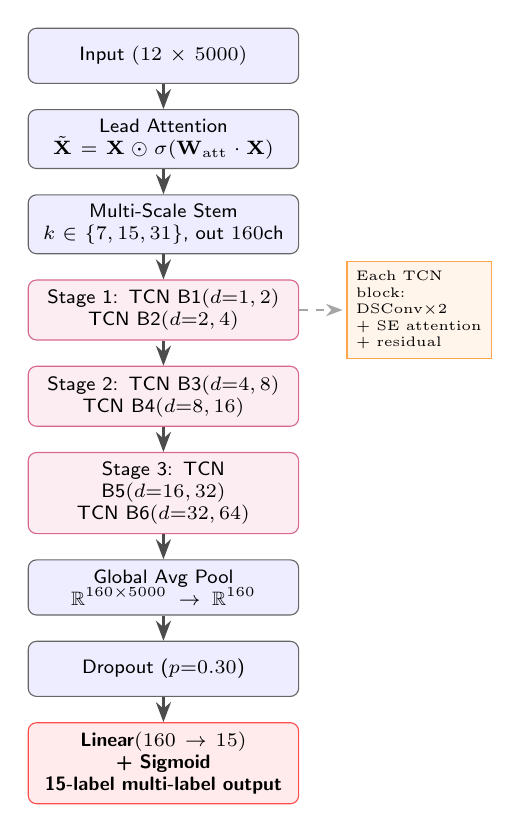
\begin{tikzpicture}[node distance=0.32cm]
  \node[flowbox, text width=3.2cm] (inp)
        {Input $(12 \times 5000)$};
  \node[flowbox, text width=3.2cm, below=of inp] (la)
        {Lead Attention\\ $\tilde{\mathbf{X}} = \mathbf{X}\odot\sigma(\mathbf{W}_{\mathrm{att}}\cdot\mathbf{X})$};
  \node[flowbox, text width=3.2cm, below=of la] (stem)
        {Multi-Scale Stem\\ $k\in\{7,15,31\}$, out $160$ch};
  \node[nbbox, text width=3.2cm, below=of stem] (s1)
        {Stage 1: TCN B1$(d{=}1,2)$\\ TCN B2$(d{=}2,4)$};
  \node[nbbox, text width=3.2cm, below=of s1] (s2)
        {Stage 2: TCN B3$(d{=}4,8)$\\ TCN B4$(d{=}8,16)$};
  \node[nbbox, text width=3.2cm, below=of s2] (s3)
        {Stage 3: TCN B5$(d{=}16,32)$\\ TCN B6$(d{=}32,64)$};
  \node[flowbox, text width=3.2cm, below=of s3] (gap)
        {Global Avg Pool\\ $\mathbb{R}^{160\times5000}\to\mathbb{R}^{160}$};
  \node[flowbox, text width=3.2cm, below=of gap] (drop)
        {Dropout ($p{=}0.30$)};
  \node[critbox, text width=3.2cm, below=of drop] (clf)
        {Linear$(160\!\to\!15)$ + Sigmoid\\ 15-label multi-label output};

  \draw[arrow] (inp)--(la);
  \draw[arrow] (la)--(stem);
  \draw[arrow] (stem)--(s1);
  \draw[arrow] (s1)--(s2);
  \draw[arrow] (s2)--(s3);
  \draw[arrow] (s3)--(gap);
  \draw[arrow] (gap)--(drop);
  \draw[arrow] (drop)--(clf);

  %% SE annotation
  \node[patnode, right=0.6cm of s1, font=\tiny, text width=1.6cm, align=left]
        {Each TCN block:\\ DSConv$\times 2$\\ + SE attention\\ + residual};
  \draw[darrow] (s1.east) -- ++(0.55,0);
\end{tikzpicture}
\caption{LightV2 architecture. Each TCN block contains two
depthwise-separable convolutions with growing dilation, a
Squeeze-and-Excitation channel attention module, and a residual
connection. Total: ${\approx}362$K parameters.}
\label{fig:model_arch}
\end{figure}

\subsection{Lead Attention Module}

A per-lead attention gate is applied as the first operation on the
raw input tensor $\mathbf{X} \in \mathbb{R}^{12 \times 5000}$:
\begin{equation}
  \tilde{\mathbf{X}} = \mathbf{X} \odot
  \sigma\!\left(\mathbf{W}_{\text{att}} \cdot \mathbf{X}\right),
\end{equation}
where $\mathbf{W}_{\text{att}}$ is a depth-wise $1{\times}1$
convolution applied independently per lead, and $\odot$ is
element-wise multiplication.
This gate learns to emphasize diagnostically relevant leads
(e.g., V1–V2 for Brugada pattern; II, III, aVF for inferior
STEMI) over less informative leads for each condition.

\subsection{Multi-Scale Convolutional Stem}

Three parallel convolutional branches with kernel sizes $k \in \{7, 15, 31\}$
capture short-range (${\sim}14$\,ms), medium-range (${\sim}30$\,ms),
and long-range (${\sim}62$\,ms) temporal dependencies respectively
(at 500\,Hz).
Each branch produces 64 feature maps:
\begin{equation}
  \mathbf{F}_k = \text{GELU}\!\left(\text{BN}\!\left(
  \mathbf{W}_k * \tilde{\mathbf{X}}\right)\right),
  \quad k \in \{7, 15, 31\},
\end{equation}
where $\mathbf{W}_k \in \mathbb{R}^{64 \times 12 \times k}$.
The three branches are concatenated and projected to 160 channels
via a pointwise $1{\times}1$ convolution:
\begin{equation}
  \mathbf{H}_0 = \text{GELU}\!\left(\text{BN}\!\left(
  \mathbf{W}_{1\times1} \cdot
  [\mathbf{F}_7 \,\|\, \mathbf{F}_{15} \,\|\, \mathbf{F}_{31}]
  \right)\right) \in \mathbb{R}^{160 \times 5000}.
\end{equation}

\subsection{Depthwise-Separable TCN Blocks}

Six temporal convolutional blocks are organized into three stages
with exponentially growing dilation factors (Table~\ref{tab:tcn}).
Each block applies two sequential depthwise-separable convolutions
(DSConv) with a squeeze-and-excitation (SE) channel attention module
\cite{hu2018squeeze} and a residual connection:
\begin{equation}
  \mathbf{H}_{l+1} = \mathbf{H}_l + \text{SE}\!\left(
  \text{BN}\!\left(\text{DSConv}_{d_{l,2}}\!\left(
  \text{DSConv}_{d_{l,1}}\!\left(\mathbf{H}_l\right)
  \right)\right)\right),
\end{equation}
where $d_{l,1}$ and $d_{l,2}$ are the two dilation factors for
block $l$ (Table~\ref{tab:tcn}).
A DSConv layer decomposes a standard convolution into a
depth-wise convolution (applied independently per channel) followed
by a point-wise $1{\times}1$ convolution, reducing parameter count
from $O(C^2 k)$ to $O(Ck + C^2)$ while preserving representational
capacity.

\begin{table}[!t]
\centering
\caption{LightV2 TCN Stage Configuration}
\label{tab:tcn}
\begin{tabular}{@{}ccccc@{}}
  \toprule
  Stage & Block & Dilation ($d_1$) & Dilation ($d_2$) & Kernel \\
  \midrule
  1 & B1 & 1  & 2  & 7 \\
  1 & B2 & 2  & 4  & 7 \\
  2 & B3 & 4  & 8  & 7 \\
  2 & B4 & 8  & 16 & 7 \\
  3 & B5 & 16 & 32 & 7 \\
  3 & B6 & 32 & 64 & 7 \\
  \bottomrule
\end{tabular}
\end{table}

\subsection{Classifier Head}

After Stage\,3, global average pooling reduces the temporal dimension:
\begin{equation}
  \mathbf{z} = \frac{1}{5000} \sum_{t=1}^{5000}
  \mathbf{H}_6[:, t] \in \mathbb{R}^{160}.
\end{equation}
Dropout ($p{=}0.30$) and a linear layer map to $L{=}15$ logits,
followed by an independent sigmoid for multi-label prediction:
\begin{equation}
  P_{\text{AI}}(D_j) = \sigma\!\left(\mathbf{w}_j^\top \mathbf{z}
  + b_j\right), \quad j = 1, \dots, 15.
\end{equation}
The total parameter count is approximately 362K (checkpoint: 1.45\,MB
in PyTorch folder format, 144 tensor files).

%% ============================================================
\section{Clinical Ontology Design}
\label{sec:ontology}

\subsection{Label Taxonomy}

The ECGenius ontology defines 35 nodes organized in a three-level
hierarchy: one root node (\texttt{ROOT}), five category nodes, and
29 leaf nodes (Fig.~\ref{fig:ontology}).
Of the 29 leaf nodes, 22 are \emph{diagnostic labels} and 7 are
\emph{ECG pattern trigger nodes} that serve as rule-engine
inputs but are not surfaced as standalone diagnoses.
Table~\ref{tab:categories} summarizes the five diagnostic categories.

\begin{table}[!t]
\centering
\caption{ECGenius Ontology: Diagnostic Categories and Label Counts}
\label{tab:categories}
\begin{tabular}{@{}lcp{4.5cm}@{}}
  \toprule
  Category    & Leaf Labels & Representative Conditions \\
  \midrule
  Rhythm      & 8  & AF, NSR, VF, VT, SVT, Atrial Flutter,
                     Sinus Bradycardia/Tachycardia \\
  Ischemia    & 3  & STEMI, NSTEMI, Unstable Angina \\
  Structural  & 5  & LVH, LVH-Strain, Pericarditis, Long QT,
                     Brugada \\
  Conduction  & 6  & LBBB, RBBB, AV Block 1\textsuperscript{st}/2\textsuperscript{nd}/3\textsuperscript{rd} \\
  ECG Pattern & 7  & ST elevation/depression, Wide QRS, TWI,
                     Irregular R-R, Short PR, PVC \\
  \midrule
  \textbf{Total} & \textbf{29} & \\
  \bottomrule
\end{tabular}
\end{table}

\begin{figure}[!t]
\centering
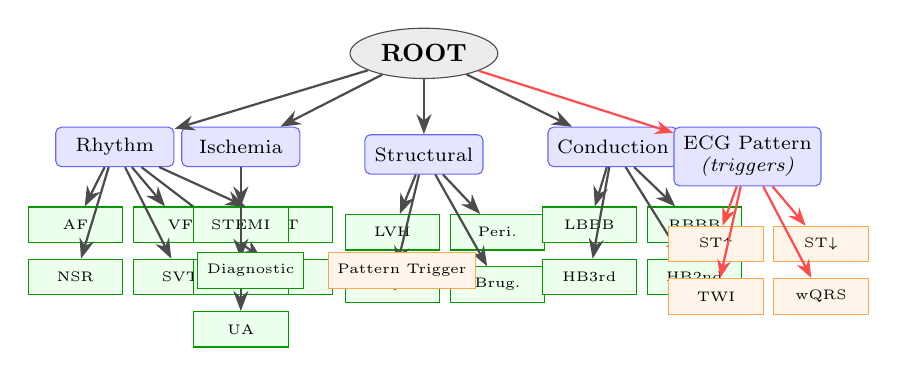
\begin{tikzpicture}[node distance=0.32cm and 0.20cm,
                    every node/.style={font=\tiny}]

  %% Root
  \node[rootnode] (root) {\small ROOT};

  %% Category row
  \node[catnode, below left=0.70cm and 2.50cm of root]  (rhy)  {Rhythm};
  \node[catnode, below left=0.70cm and 0.90cm of root]  (isc)  {Ischemia};
  \node[catnode, below=0.70cm of root]                  (str)  {Structural};
  \node[catnode, below right=0.70cm and 0.90cm of root] (con)  {Conduction};
  \node[catnode, below right=0.70cm and 2.50cm of root] (pat)  {ECG Pattern\\\textit{(triggers)}};

  \draw[arrow] (root) -- (rhy);
  \draw[arrow] (root) -- (isc);
  \draw[arrow] (root) -- (str);
  \draw[arrow] (root) -- (con);
  \draw[rarrow] (root) -- (pat);

  %% Rhythm leaves
  \node[leafnode, below=0.50cm of rhy, xshift=-0.50cm] (af)   {AF};
  \node[leafnode, right=0.12cm of af]                   (vf)   {VF};
  \node[leafnode, right=0.12cm of vf]                   (vt)   {VT};
  \node[leafnode, below=0.20cm of af]                   (nsr)  {NSR};
  \node[leafnode, right=0.12cm of nsr]                  (svt)  {SVT};
  \node[leafnode, right=0.12cm of svt]                  (sb)   {SB};
  \draw[arrow] (rhy) -- (af); \draw[arrow] (rhy) -- (vf);
  \draw[arrow] (rhy) -- (vt); \draw[arrow] (rhy) -- (nsr);
  \draw[arrow] (rhy) -- (svt); \draw[arrow] (rhy) -- (sb);

  %% Ischemia leaves
  \node[leafnode, below=0.50cm of isc] (stemi)  {STEMI};
  \node[leafnode, below=0.20cm of stemi] (nstemi) {NSTEMI};
  \node[leafnode, below=0.20cm of nstemi] (ua)  {UA};
  \draw[arrow] (isc) -- (stemi);
  \draw[arrow] (isc) -- (nstemi);
  \draw[arrow] (isc) -- (ua);

  %% Structural leaves
  \node[leafnode, below=0.50cm of str, xshift=-0.40cm] (lvh)  {LVH};
  \node[leafnode, right=0.12cm of lvh]                  (peri) {Peri.};
  \node[leafnode, below=0.20cm of lvh]                  (lqt)  {LQT};
  \node[leafnode, right=0.12cm of lqt]                  (brug) {Brug.};
  \draw[arrow] (str) -- (lvh);  \draw[arrow] (str) -- (peri);
  \draw[arrow] (str) -- (lqt);  \draw[arrow] (str) -- (brug);

  %% Conduction leaves
  \node[leafnode, below=0.50cm of con, xshift=-0.30cm] (lbbb) {LBBB};
  \node[leafnode, right=0.12cm of lbbb]                 (rbbb) {RBBB};
  \node[leafnode, below=0.20cm of lbbb]                 (hb3)  {HB3rd};
  \node[leafnode, right=0.12cm of hb3]                  (hb2)  {HB2nd};
  \draw[arrow] (con) -- (lbbb); \draw[arrow] (con) -- (rbbb);
  \draw[arrow] (con) -- (hb3);  \draw[arrow] (con) -- (hb2);

  %% Pattern trigger leaves (orange)
  \node[patnode, below=0.50cm of pat, xshift=-0.40cm] (ste)  {ST$\uparrow$};
  \node[patnode, right=0.12cm of ste]                   (std)  {ST$\downarrow$};
  \node[patnode, below=0.20cm of ste]                   (twi)  {TWI};
  \node[patnode, right=0.12cm of twi]                   (wqrs) {wQRS};
  \draw[rarrow] (pat) -- (ste);  \draw[rarrow] (pat) -- (std);
  \draw[rarrow] (pat) -- (twi);  \draw[rarrow] (pat) -- (wqrs);

  %% Legend
  \node[leafnode, below=2.20cm of root, xshift=-2.2cm]  (leg1) {Diagnostic};
  \node[patnode,  right=0.30cm of leg1]                  (leg2) {Pattern Trigger};

\end{tikzpicture}
\caption{ECGenius ontology hierarchy (simplified). Orange nodes are
ECG pattern triggers used exclusively as rule-engine inputs.
\textit{SB}: Sinus Bradycardia; \textit{Peri.}: Pericarditis;
\textit{Brug.}: Brugada; \textit{HB3rd/2nd}: Heart Block 3rd/2nd degree;
\textit{ST$\uparrow$/$\downarrow$}: ST elevation/depression;
\textit{wQRS}: Wide QRS; \textit{TWI}: T-wave inversion.}
\label{fig:ontology}
\end{figure}

\subsection{Triage Classification}

Every diagnostic label carries a clinical urgency tier:
\textbf{Tier\,1} (life-threatening), \textbf{Tier\,2} (urgent),
or \textbf{Tier\,3} (routine).
Tier-1 labels---STEMI, VF, VT, NSTEMI, Complete AV Block
(Heart\_Block\_3rd), Mobitz~II (Heart\_Block\_2nd\_MobitzII),
and Brugada---trigger absolute safety overrides (Section~\ref{sec:fusion}).
Each label also carries a default clinical action (e.g.,
\textit{``Immediate PCI referral — door-to-balloon $<$90\,min''} for
STEMI) and an \texttt{allow\_downgrade} flag.

\subsection{Standard Terminology Mappings}

All 22 diagnostic leaf labels are mapped to:
(i) SNOMED-CT concept identifiers \cite{snomedct}
    (e.g., STEMI $\to$ 57054005);
(ii) ICD-10-CM codes \cite{icd10}
    (e.g., STEMI anterior $\to$ I21.0);
(iii) AHA/ACC guideline identifiers
    (e.g., STEMI $\to$ 2013\_AHA\_STEMI\_Guideline \cite{ogara2013stemi}).
These mappings are stored in \texttt{ontology/mappings.csv} and
exposed in the system output JSON for direct EHR integration.

%% ============================================================
\section{Rule-Based Clinical Reasoning}
\label{sec:rules}

\subsection{Rule Engine Architecture}

The rule engine is decoupled from the inference pipeline via a
CSV-driven handler registry.
Rules are defined in \texttt{ontology/rules.csv} and loaded at
startup; adding a new rule requires no code changes.
Rule handlers are registered via a decorator pattern:
\texttt{@register(\textit{rule\_type})},
enabling new rule types to be added by dropping a Python module
into \texttt{rule\_definitions/}.
Fig.~\ref{fig:rules} illustrates the rule execution workflow.

\begin{figure}[!t]
\centering
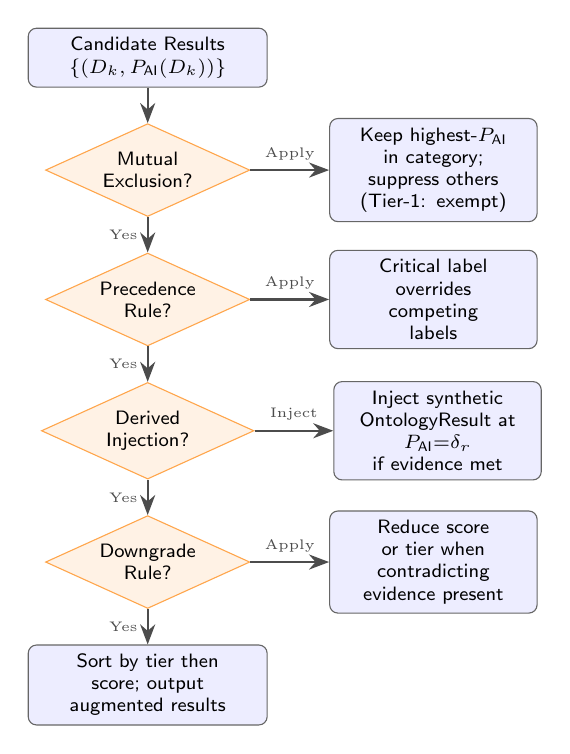
\begin{tikzpicture}[node distance=0.40cm]

  \node[flowbox, text width=2.8cm] (inp)
        {Candidate Results\\ $\{(D_k, P_{\text{AI}}(D_k))\}$};

  \node[decision, below=0.45cm of inp] (me)
        {Mutual\\ Exclusion?};

  \node[flowbox, right=1.0cm of me, text width=2.4cm] (meact)
        {Keep highest-$P_{\text{AI}}$\\ in category;\\ suppress others\\ (Tier-1: exempt)};

  \node[decision, below=0.45cm of me] (pre)
        {Precedence\\ Rule?};

  \node[flowbox, right=1.0cm of pre, text width=2.4cm] (preact)
        {Critical label\\ overrides\\ competing\\ labels};

  \node[decision, below=0.45cm of pre] (der)
        {Derived\\ Injection?};

  \node[flowbox, right=1.0cm of der, text width=2.4cm] (deract)
        {Inject synthetic\\ OntologyResult at\\ $P_{\text{AI}}{=}\delta_r$\\ if evidence met};

  \node[decision, below=0.45cm of der] (dng)
        {Downgrade\\ Rule?};

  \node[flowbox, right=1.0cm of dng, text width=2.4cm] (dngact)
        {Reduce score\\ or tier when\\ contradicting\\ evidence present};

  \node[flowbox, text width=2.8cm, below=0.45cm of dng] (out)
        {Sort by tier then\\ score; output\\ augmented results};

  %% Main flow
  \draw[arrow] (inp) -- (me);
  \draw[arrow] (me)  -- node[left,font=\tiny]{Yes} (pre);
  \draw[arrow] (me)  -- node[above,font=\tiny]{Apply} (meact);
  \draw[arrow] (pre) -- node[left,font=\tiny]{Yes} (der);
  \draw[arrow] (pre) -- node[above,font=\tiny]{Apply} (preact);
  \draw[arrow] (der) -- node[left,font=\tiny]{Yes} (dng);
  \draw[arrow] (der) -- node[above,font=\tiny]{Inject} (deract);
  \draw[arrow] (dng) -- node[left,font=\tiny]{Yes} (out);
  \draw[arrow] (dng) -- node[above,font=\tiny]{Apply} (dngact);

  %% No arrows (straight down already implied by main flow)

\end{tikzpicture}
\caption{Rule engine execution workflow. Each rule type is handled
by a registered Python function. Execution continues through all
rule types regardless of prior matches. Exception handling ensures
that a single rule failure does not terminate the pipeline.}
\label{fig:rules}
\end{figure}

\subsection{Rule Categories}

\subsubsection{Mutual Exclusion}
Clinically, a patient can exhibit only one dominant rhythm at a
given moment.
Rule~R1 keeps the rhythm label with the highest $P_{\text{AI}}$
within the \texttt{Rhythm} category and marks all others as
\texttt{is\_suppressed=True}.
A critical safety exception applies: Tier-1 rhythm labels (VF, VT)
are \emph{never} suppressed regardless of their relative probability.

\subsubsection{Precedence}
Four precedence rules encode clinical severity hierarchies:
\begin{itemize}
  \item R2a: VF overrides all other rhythm labels (cardiac arrest
        renders them clinically irrelevant).
  \item R2b: VT overrides Sinus Bradycardia, Sinus Tachycardia,
        and NSR.
  \item R2c: Complete AV Block (3rd degree) overrides all lower-degree
        AV blocks.
  \item R2d: Mobitz~II overrides Wenckebach (Mobitz~I) and
        1st-degree AV Block.
\end{itemize}

\subsubsection{Derived Diagnosis Injection}
\label{sec:derived}
Pattern trigger nodes serve as intermediate ECG findings that are
below the diagnostic threshold but clinically imply a specific
diagnosis when combined with patient evidence.
Five derived-injection rules are defined (Table~\ref{tab:derived}).
The rule mechanism prevents clinically critical diagnoses from being
missed due to a model's lower-than-threshold probability estimate.

\begin{table}[!t]
\centering
\caption{Derived Diagnosis Injection Rules}
\label{tab:derived}
\setlength{\tabcolsep}{3pt}
\begin{tabular}{@{}lllcc@{}}
  \toprule
  Rule & Trigger & Required Evidence & Injected Dx & $\delta_r$ \\
  \midrule
  R3b & ST Elevation & (none)       & Pericarditis      & 0.20 \\
  R4b & ST Depression & (none)      & Unstable Angina   & 0.18 \\
  R7  & LBBB         & chest pain   & STEMI\textsuperscript{a} & 0.40 \\
  V2  & TWI          & chest pain   & NSTEMI\textsuperscript{b} & 0.35 \\
  V8  & Long QT      & palpitations & VT\textsuperscript{c}     & 0.30 \\
  \bottomrule
\end{tabular}\\[2pt]
\raggedright
\footnotesize
$^a$ Sgarbossa criterion \cite{sgarbossa1996electrocardiographic}: LBBB
     with chest pain constitutes a STEMI-equivalent requiring emergent
     reperfusion.\\
$^b$ Wellens Pattern A \cite{zwaan1989wellens}: deep T-wave inversions
     in V2-V3 with chest pain indicate critical LAD stenosis.\\
$^c$ Torsades de Pointes risk: QTc prolongation with palpitations
     requires immediate evaluation for VT.
\end{table}

\subsubsection{Downgrade Rules}
The system architecture supports downgrade rules that reduce the
confidence tier of a diagnosis when contradicting clinical evidence
is present (e.g., STEMI tier reduced when chest pain is absent and
the finding is an incidental electrocardiographic pattern).
This rule type is defined in the handler registry but has no entries
in the current \texttt{rules.csv}, representing a planned extension
for cardiologist-validated deployment.

\subsection{Safety Guarantees}
Two safety properties are enforced by the rule engine:
\begin{enumerate}
  \item \textbf{Tier-1 Non-Suppression}: The mutual exclusion handler
        explicitly checks and refuses to suppress any label whose
        triage tier is 1, logging a warning if suppression is
        attempted.
  \item \textbf{Rule Fault Isolation}: Each rule execution is wrapped
        in a try-except block; a failing rule logs an error and is
        skipped without interrupting the pipeline.
\end{enumerate}

%% ============================================================
\section{Patient History Encoder}
\label{sec:history}

The history encoder transforms a structured patient record into
a per-label evidence dictionary suitable for Bayesian fusion.
Three evidence types are supported:
\begin{itemize}
  \item \textbf{Symptoms}: binary flags (e.g., \texttt{chest\_pain},
        \texttt{dyspnea}, \texttt{palpitations}).
  \item \textbf{Risk Factors}: binary flags (e.g., \texttt{cad},
        \texttt{dm}, \texttt{htn}, \texttt{smoking},
        \texttt{prior\_mi}).
  \item \textbf{Vital Signs}: continuous values thresholded into
        binary flags (Table~\ref{tab:vitals}).
\end{itemize}

\begin{table}[!t]
\centering
\caption{Vital Sign Threshold Flags}
\label{tab:vitals}
\begin{tabular}{@{}lll@{}}
  \toprule
  Vital & Flag & Clinical Significance \\
  \midrule
  SBP & \texttt{sbp\_lt\_70/90/100}  & Hypotension / cardiogenic shock \\
      & \texttt{sbp\_gt\_140/160}    & Hypertension \\
  HR  & \texttt{hr\_lt\_40/60}       & Bradycardia / complete block \\
      & \texttt{hr\_gt\_100/150/160/200} & Tachycardia \\
  SpO\textsubscript{2}
      & \texttt{spo2\_lt\_94}        & Hypoxia / pulmonary edema \\
  \bottomrule
\end{tabular}
\end{table}

\subsection{Conditional Probability Tables}

The history encoder loads \texttt{history\_rules.csv}, which
encodes a conditional probability table (CPT) with 98 entries
covering 20 diagnostic conditions.
Each entry specifies $P(E_i \,|\, D_k)$ and
$P(E_i \,|\, \neg D_k)$ for a specific
(disease, evidence) pair.
Table~\ref{tab:cpt_sample} shows representative entries for STEMI.

\begin{table}[!t]
\centering
\caption{CPT Sample: STEMI Evidence Associations}
\label{tab:cpt_sample}
\begin{tabular}{@{}llccc@{}}
  \toprule
  Rule & Evidence Feature & $P(E\,|\,D)$ & $P(E\,|\,\neg D)$ & LR \\
  \midrule
  H1  & chest\_pain    & 0.88 & 0.15 & 5.87 \\
  H2  & diaphoresis    & 0.52 & 0.08 & 6.50 \\
  H5  & cad            & 0.60 & 0.20 & 3.00 \\
  H9  & sbp\_lt\_90    & 0.22 & 0.04 & 5.50 \\
  H11 & hr\_gt\_100    & 0.35 & 0.12 & 2.92 \\
  H6  & dm             & 0.28 & 0.18 & 1.56 \\
  \bottomrule
\end{tabular}\\[2pt]
\raggedright
\footnotesize
LR: Likelihood Ratio $= P(E\,|\,D) / P(E\,|\,\neg D)$.
Values initialized from clinical literature (Framingham, INTERHEART,
ESC guidelines). Recalibration on the AIIMS Nagpur cohort is planned
as Phase\,3 work.
\end{table}

The CPT values in the current implementation are initialized from
published clinical epidemiology studies
\cite{antman2004acc,yusuf2004interheart} and have not yet been
calibrated on the AIIMS Nagpur Indian cohort.
Recalibration via Maximum Likelihood Estimation using \texttt{pgmpy}
or \texttt{bnlearn} is planned for Phase\,3 of the project.

%% ============================================================
\section{Bayesian Decision Fusion}
\label{sec:fusion}

\subsection{Problem Formulation}

Let $\mathcal{D} = \{D_1, \ldots, D_K\}$ be the set of candidate
diagnoses present in the ontology results after rule execution.
Let $\mathcal{E} = \{E_1, \ldots, E_N\}$ be the set of active
patient evidence features.
The goal of decision fusion is to compute, for each diagnosis $D_k$:
\begin{equation}
  P(D_k \,|\, \mathcal{E}) \propto
  P(D_k) \cdot \prod_{i=1}^{N} \frac{P(E_i \,|\, D_k)}{P(E_i \,|\, \neg D_k)},
  \label{eq:nb_full}
\end{equation}
where $P(D_k)$ is the prior probability provided by the AI model
(normalized across candidates) and the product terms are
likelihood ratios (LR) from the CPT table.
The conditional independence assumption $E_i \perp E_j \,|\, D_k$
is adopted, which is the Naive Bayes assumption.

\subsection{Log-Space Implementation}

Direct multiplication of probabilities leads to numerical underflow
for long evidence chains.
ECGenius implements the fusion in log-space:
\begin{equation}
  \text{Score}(D_k) = \log P(D_k) + \sum_{i=1}^{N}
  \underbrace{\log\!\left[\frac{P(E_i \,|\, D_k)}{P(E_i \,|\, \neg D_k)}\right]}_{\log\,\text{LR}_i(D_k)},
  \label{eq:log_score}
\end{equation}
where only \emph{active} evidence features ($E_i = \texttt{True}$)
contribute to the sum.
Laplace smoothing $\varepsilon = 10^{-6}$ is applied to all CPT
values to prevent $\log(0)$.
Numerical stability is enforced by subtracting the maximum log-score
before exponentiation:
\begin{equation}
  P(D_k \,|\, \mathcal{E}) = \frac{%
  \exp\!\left(\text{Score}(D_k) - \max_{j} \text{Score}(D_j)\right)}{%
  \sum_{j=1}^{K}
  \exp\!\left(\text{Score}(D_j) - \max_{j'} \text{Score}(D_{j'})\right)}.
  \label{eq:softmax_stable}
\end{equation}
Pattern category nodes (ST elevation, T-wave inversion, etc.) are
excluded from the set of prior inputs $\mathcal{D}$, as they are
rule triggers rather than diagnostic hypotheses.

\subsection{Confidence Tier Assignment}
\label{sec:confidence}

Posterior probabilities are mapped to four confidence labels:
\begin{equation}
  \text{Conf}(D_k) =
  \begin{cases}
    \textsc{Confirmed}   & P(D_k \,|\, \mathcal{E}) \geq 0.80, \\
    \textsc{Probable}    & 0.60 \leq P(D_k \,|\, \mathcal{E}) < 0.80, \\
    \textsc{Possible}    & 0.30 \leq P(D_k \,|\, \mathcal{E}) < 0.60, \\
    \textsc{Incidental}  & P(D_k \,|\, \mathcal{E}) < 0.30.
  \end{cases}
  \label{eq:conf}
\end{equation}
These thresholds are design decisions of the current system and
are subject to calibration against clinical outcome data.

\subsection{Tier-1 Safety Override}

For Tier-1 life-threatening diagnoses, an additional safety rule
prevents under-reporting:
\begin{equation}
  \text{Conf}(D_k) = \textsc{Confirmed}
  \quad \text{if} \quad D_k \in \mathcal{T}_1
  \;\text{and}\; P(D_k \,|\, \mathcal{E}) > 0.15,
  \label{eq:t1_override}
\end{equation}
where $\mathcal{T}_1 = \{\text{STEMI},\, \text{VF},\, \text{VT}\}$
for the Naive Bayes path.
For all Tier-1 labels from the triage table in the legacy scoring
path, an \textsc{Incidental} rating is elevated to \textsc{Possible},
and a \textsc{Possible} rating is elevated to \textsc{Probable} when
$P_{\text{AI}}(D_k) \geq 0.70$.
This asymmetric sensitivity policy is a deliberate design choice
prioritizing clinical recall over precision for critical conditions.

The complete fusion procedure is formalized in
Algorithm~\ref{alg:fusion} and illustrated in
Fig.~\ref{fig:bayesian}.

\begin{algorithm}[t]
\caption{ECGenius Naive Bayesian Decision Fusion}
\label{alg:fusion}
\begin{algorithmic}[1]
  \REQUIRE AI priors $\{P_{\text{AI}}(D_k)\}$, patient evidence
           $\mathcal{E}$, CPT table, tier-1 set $\mathcal{T}_1$
  \ENSURE  Ranked differential diagnosis $\{(D_k,\,
           P(D_k|\mathcal{E}),\, \text{Conf}_k)\}$

  \STATE Normalize: $P(D_k) \leftarrow P_{\text{AI}}(D_k)
         \,/\, \sum_j P_{\text{AI}}(D_j)$
  \STATE Build CPT index: $(D_k, E_i) \to (p^+_{ki}, p^-_{ki})$
  \FOR{each candidate $D_k$}
    \STATE $s_k \leftarrow \log P(D_k)$
    \FOR{each active feature $E_i \in \mathcal{E}$}
      \IF{$(D_k, E_i)$ in CPT index}
        \STATE $s_k \mathrel{+}= \log\!\big(
               \max(p^+_{ki}, \varepsilon) \,/\,
               \max(p^-_{ki}, \varepsilon)\big)$
      \ENDIF
    \ENDFOR
  \ENDFOR
  \STATE $s^* \leftarrow \max_k s_k$
  \STATE $w_k \leftarrow \exp(s_k - s^*)\; \forall k$
  \STATE $P(D_k|\mathcal{E}) \leftarrow w_k \,/\, \sum_j w_j$
  \STATE Assign $\text{Conf}_k$ via (\ref{eq:conf})
  \STATE Apply Tier-1 override via (\ref{eq:t1_override})
  \STATE Sort by $P(D_k|\mathcal{E})$ descending; assign ranks
  \RETURN Ranked DDx list
\end{algorithmic}
\end{algorithm}

\begin{figure}[!t]
\centering
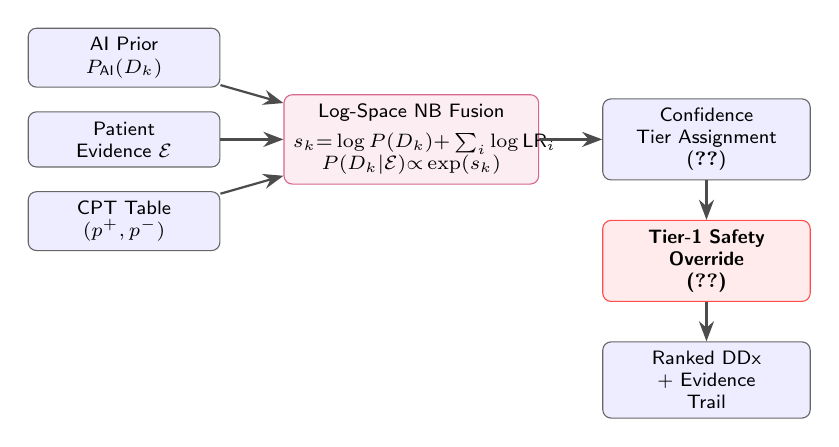
\begin{tikzpicture}[node distance=0.38cm and 0.30cm]

  %% Input nodes
  \node[flowbox, text width=2.2cm] (prior) {AI Prior\\ $P_{\text{AI}}(D_k)$};
  \node[flowbox, text width=2.2cm, below=0.30cm of prior] (ev)
        {Patient\\ Evidence $\mathcal{E}$};
  \node[flowbox, text width=2.2cm, below=0.30cm of ev] (cpt)
        {CPT Table\\ $(p^+, p^-)$};

  %% NB engine
  \node[nbbox, text width=3.0cm,
        right=0.80cm of ev] (nb)
        {Log-Space NB Fusion\\[3pt]
         $s_k{=}\log P(D_k){+}\sum_i\log\text{LR}_i$\\
         $P(D_k|\mathcal{E}){\propto}\exp(s_k)$};

  \draw[arrow] (prior) -- (nb);
  \draw[arrow] (ev)    -- (nb);
  \draw[arrow] (cpt)   -- (nb);

  %% Confidence assignment
  \node[flowbox, text width=2.4cm, right=0.80cm of nb] (conf)
        {Confidence\\ Tier Assignment\\ (\ref{eq:conf})};
  \draw[arrow] (nb) -- (conf);

  %% Safety override
  \node[critbox, text width=2.4cm,
        below=0.50cm of conf] (safe)
        {Tier-1 Safety\\ Override\\ (\ref{eq:t1_override})};
  \draw[arrow] (conf) -- (safe);

  %% Output
  \node[flowbox, text width=2.4cm, below=0.50cm of safe] (out)
        {Ranked DDx\\ + Evidence\\ Trail};
  \draw[arrow] (safe) -- (out);

  %% Brace annotations
  \node[right=0.1cm of nb, font=\tiny, align=left,
        yshift=0.25cm] {};

\end{tikzpicture}
\caption{Bayesian decision fusion workflow. Three information sources
(AI prior, patient evidence, CPT likelihood ratios) are combined in
log-space. Confidence tiers are assigned and then conditionally
overridden for Tier-1 life-threatening diagnoses.}
\label{fig:bayesian}
\end{figure}

\subsection{Legacy Fallback Mode}

For backward compatibility with earlier CSV schemas, a weighted
additive fallback is provided:
\begin{equation}
  \text{Score}^{\text{legacy}}(D_k) =
  \underbrace{\tfrac{1}{2} \hat{P}_{\text{AI}}(D_k)}_{S_{\text{AI}}}
  + \underbrace{S_{\text{sym}}(D_k)}_{\leq 0.30}
  + \underbrace{S_{\text{risk}}(D_k)}_{\leq 0.10}
  + \underbrace{S_{\text{rule}}(D_k)}_{\leq 0.10},
  \label{eq:legacy}
\end{equation}
where $\hat{P}_{\text{AI}}(D_k) = P_{\text{AI}}(D_k) / \sum_j P_{\text{AI}}(D_j)$.
This fallback is activated automatically when the CPT table is
detected to contain legacy \texttt{action}/\texttt{delta} columns
rather than the \texttt{p\_given\_disease}/\texttt{p\_given\_not\_disease}
schema.

%% ============================================================
\section{Explainability Framework}
\label{sec:explainability}

\subsection{Score Decomposition}

For each diagnosis in the fusion output, ECGenius records a
structured score breakdown:
\texttt{pai} (raw model probability),
\texttt{s\_ai} (normalized prior),
\texttt{nb\_breakdown} (log-prior, log-likelihood, per-feature LR terms),
and, in legacy mode, \texttt{s\_symptom}, \texttt{s\_risk}, \texttt{s\_rule}.
These values are stored in the \texttt{FusionResult} dataclass and
serialized to JSON, enabling downstream audit without access to
model internals.

\subsection{Likelihood Ratio Narratives}

The NB breakdown exposes per-evidence likelihood ratio contributions
$\log\,\text{LR}_i(D_k)$ for every active feature.
Evidence with $\text{LR} > 1$ is classified as ``supporting'' the
diagnosis; evidence with $\text{LR} < 1$ is classified as
``contradicting.''
These signed lists are exposed as \texttt{supporting} and
\texttt{contradicting} fields in the output, enabling a clinician
to review which patient features most influenced each ranked
diagnosis.

\subsection{Per-Diagnosis Audit Trail}

The explainability module generates a structured audit trail per
diagnosis containing:
(i) raw AI probability and normalized prior;
(ii) score computation steps (for legacy: equation~\ref{eq:legacy};
     for NB: equation~\ref{eq:log_score});
(iii) triage tier and default clinical action;
(iv) SNOMED-CT, ICD-10, and AHA guideline identifiers;
(v) supporting and contradicting evidence lists;
(vi) derived rule contributions (e.g., which Sgarbossa rule triggered
a STEMI injection and from which ECG pattern).

\subsection{Clinical Narrative Generation}

A short natural-language narrative is synthesized from the audit
trail for each diagnosis.
Example: for STEMI with $P_{\text{AI}} = 0.74$ and derived injection
from LBBB+chest\_pain:
\begin{quote}
\textit{``[CRITICAL] ST-Elevation MI is strongly supported (posterior
0.80). ECG pattern strongly detected (AI probability 74.0\%).
Clinical symptoms: chest pain, diaphoresis. STEMI surfaced by
Sgarbossa derived rule (trigger: LBBB + chest\_pain). Recommended
action: Immediate PCI referral — door-to-balloon $<$90\,min.''}
\end{quote}
Narratives are generated by rule-based string templates applied to
the structured audit data, ensuring reproducibility and
auditability.

%% ============================================================
\section{Implementation Details}
\label{sec:impl}

\subsection{Software Stack}

ECGenius is implemented in Python 3.10+.
The neural network uses PyTorch 2.x with \texttt{torch.no\_grad()}
inference and automatic CUDA/MPS/CPU device selection.
Signal processing uses \texttt{scipy.signal} (Butterworth filter,
IIR notch, resample).
Ontology and CPT tables are loaded from CSV via \texttt{pandas}.
The web API uses FastAPI with \texttt{uvicorn} and exposes REST
endpoints for single-ECG and batch inference.
The frontend is a React application communicating with the API over
HTTP.

\subsection{Model Specifications}

Table~\ref{tab:model_spec} summarizes the LightV2 model
specifications.

\begin{table}[!t]
\centering
\caption{LightV2 Model Specifications}
\label{tab:model_spec}
\begin{tabular}{@{}ll@{}}
  \toprule
  Property & Value \\
  \midrule
  Architecture       & Multi-scale 1D TCN + SE + Lead Attention \\
  Input shape        & $(12,\ 5000)$ at 500\,Hz \\
  Output             & 15-class sigmoid multi-label \\
  Base channels      & 160 \\
  TCN stages         & 3 stages $\times$ 2 blocks = 6 blocks \\
  Kernel size        & 7 (all TCN layers) \\
  Dilation sequence  & 1, 2, 4, 8, 16, 32 (per stage) \\
  Parameters         & ${\approx}362\,000$ \\
  Checkpoint size    & 1.45\,MB (144 tensor files, folder format) \\
  Dropout            & $p{=}0.30$ \\
  Activation         & GELU (TCN), ReLU (SE), Sigmoid (output) \\
  \bottomrule
\end{tabular}
\end{table}

The checkpoint is stored in PyTorch's folder format
(unzipped \texttt{.pt} archive: \texttt{data.pkl} + 144 tensor files).
A multi-strategy loader handles folder checkpoints, full-model
\texttt{.pt} files, state-dict \texttt{.pt} files (strict and
non-strict), and TorchScript \texttt{.pt} files, enabling
deployment-time flexibility.

\subsection{Inference Endpoint}

The \texttt{POST /diagnose} FastAPI endpoint accepts a
\texttt{DiagnoseRequest} JSON body containing:
\texttt{model\_output} (pre-computed label probabilities),
\texttt{patient} (symptoms, risk factors, vitals), and
\texttt{patient\_id}.
The response is a \texttt{FusionOutput} JSON containing
the top diagnosis, differential diagnosis list, critical alerts,
and per-diagnosis audit trails.
A \texttt{GET /schema/\{label\_id\}} endpoint returns the minimal
question set for a given diagnosis from
\texttt{history\_schema.json}, enabling adaptive history collection.

%% ============================================================
\section{Experimental Setup}
\label{sec:setup}

\subsection{Dataset Description}

Experiments are designed on two datasets.

\textbf{Dataset~1: AIIMS Nagpur Cohort.}
Approximately 40,000 12-lead ECG recordings collected at AIIMS
Nagpur Hospital, India, from inpatients and outpatients presenting
with cardiovascular symptoms.
Each recording is paired with a structured patient record
(demographics, symptoms, risk factors, vital signs) and
cardiologist-assigned diagnostic labels.
Full dataset characteristics, class distribution, and
data quality statistics will be reported in the results section.
The study is conducted with appropriate institutional ethical
approval and informed patient consent.

\textbf{Dataset~2: PhysioNet/CinC 2020-2021.}
A publicly available multi-label ECG classification benchmark
comprising recordings from 12 international ECG databases
\cite{reyna2020physionet,reyna2021physionet}.
This dataset is used for pre-training and cross-population
validation.
The \texttt{.mat} WFDB format is supported natively by the
ECGenius preprocessing pipeline.

\subsection{Data Preprocessing and Splits}

All recordings are preprocessed by the pipeline described in
Section~\ref{sec:preprocess} to produce standardized
$(12, 5000)$ float32 arrays at 500\,Hz.
Patient-level splits are performed to prevent data leakage.
Split proportions: 70\% training, 15\% validation, 15\% test.
Split indices are stored in
\texttt{data/processed/splits/\{train,val,test\}\_ids.txt}.

\subsection{Training Configuration}
\label{sec:training_config}

The LightV2 model is trained with PyTorch Lightning using the
hyperparameter configuration in Table~\ref{tab:train_config}.
Asymmetric Binary Cross-Entropy loss \cite{ridnik2021asymmetric}
is used to handle class imbalance, with $\gamma_{\text{neg}} = 4.0$.

\begin{table}[!t]
\centering
\caption{LightV2 Training Hyperparameters}
\label{tab:train_config}
\begin{tabular}{@{}ll@{}}
  \toprule
  Hyperparameter & Value \\
  \midrule
  Optimizer           & AdamW \\
  Learning rate       & $10^{-4}$ (warmup 5 epochs) \\
  Scheduler           & Cosine annealing to $10^{-6}$ \\
  Batch size          & 32 \\
  Max epochs          & 100 (early stop, patience 15) \\
  Loss function       & Asymmetric BCE ($\gamma_-{=}4.0$) \\
  Mixed precision     & FP16 \\
  Augmentation        & Gaussian noise, amplitude scaling,
                        time shift, lead dropout \\
  Class weighting     & Enabled (inverse frequency) \\
  \bottomrule
\end{tabular}
\end{table}

\subsection{Evaluation Metrics}

System evaluation employs metrics appropriate for multi-label
clinical classification:

\begin{itemize}
  \item \textbf{Per-label}: AUC-ROC, F1, Precision, Recall,
        Specificity (optimal threshold from validation set).
  \item \textbf{Macro/weighted aggregates}: AUC-ROC, F1.
  \item \textbf{Top-$K$ DDx accuracy}: fraction of cases where
        the ground-truth primary diagnosis appears in the top-1
        and top-3 ranked differential diagnoses.
  \item \textbf{Tier-1 recall}: Recall computed exclusively on
        life-threatening diagnoses ($\mathcal{T}_1$), the
        primary clinical safety metric.
  \item \textbf{Calibration}: Brier score and reliability
        diagrams for posterior probability calibration.
  \item \textbf{Explainability}: Qualitative cardiologist evaluation
        of audit trails and narratives via a structured assessment
        form (future validation study).
\end{itemize}

\subsection{Baseline Methods}

Four system variants are evaluated in an ablation study to
quantify the contribution of each component:

\begin{itemize}
  \item \textbf{Variant~A: AI Only.} LightV2 model output
        thresholded at 0.10. No ontology, rules, or history.
  \item \textbf{Variant~B: AI + Ontology.} Adds ontology mapping
        with hierarchy enrichment, triage classification, and
        mutual exclusion rules.
  \item \textbf{Variant~C: AI + Ontology + History.} Adds patient
        history encoder with CPT-based Naive Bayes fusion.
  \item \textbf{Variant~D: Full System.} Adds the clinical rule
        engine including precedence rules and derived diagnosis
        injection.
\end{itemize}

%% ============================================================
\section{Results}
\label{sec:results}

\textit{Note: Full experimental validation is ongoing.
All numerical values in this section are placeholders for
prospective results. Tables include the complete proposed structure
to facilitate direct replacement upon experiment completion.}

\subsection{Diagnostic Performance on AIIMS Cohort}

Table~\ref{tab:main_results} reports the primary diagnostic
performance metrics.

\begin{table}[!t]
\centering
\caption{Diagnostic Performance: ECGenius Full System vs.\ Baselines
         (AIIMS Nagpur Test Set)}
\label{tab:main_results}
\setlength{\tabcolsep}{3pt}
\begin{tabular}{@{}lccccc@{}}
  \toprule
  Method & AUC-ROC & F1 & Precision & Recall & Top-3 Acc. \\
  \midrule
  Variant A: AI Only        & [TBD] & [TBD] & [TBD] & [TBD] & [TBD] \\
  Variant B: + Ontology     & [TBD] & [TBD] & [TBD] & [TBD] & [TBD] \\
  Variant C: + History      & [TBD] & [TBD] & [TBD] & [TBD] & [TBD] \\
  Variant D: Full System    & [TBD] & [TBD] & [TBD] & [TBD] & [TBD] \\
  \midrule
  Human Cardiologist [TBD]  & --    & [TBD] & [TBD] & [TBD] & --    \\
  \bottomrule
\end{tabular}
\end{table}

\subsection{Per-Label Performance}

Table~\ref{tab:perlabel} reports per-label AUC-ROC and F1 scores
for the full system on the AIIMS test set.

\begin{table}[!t]
\centering
\caption{Per-Label Diagnostic Performance (Full System, AIIMS Test Set)}
\label{tab:perlabel}
\setlength{\tabcolsep}{3pt}
\begin{tabular}{@{}llccc@{}}
  \toprule
  Label & Category & AUC-ROC & F1 & Tier \\
  \midrule
  STEMI               & Ischemia   & [TBD] & [TBD] & 1 \\
  NSTEMI              & Ischemia   & [TBD] & [TBD] & 1 \\
  Unstable Angina     & Ischemia   & [TBD] & [TBD] & 2 \\
  VF                  & Rhythm     & [TBD] & [TBD] & 1 \\
  VT                  & Rhythm     & [TBD] & [TBD] & 1 \\
  AF                  & Rhythm     & [TBD] & [TBD] & 2 \\
  Heart Block 3rd     & Conduction & [TBD] & [TBD] & 1 \\
  Heart Block Mobitz II & Conduction & [TBD] & [TBD] & 1 \\
  LBBB                & Conduction & [TBD] & [TBD] & 2 \\
  Brugada             & Structural & [TBD] & [TBD] & 1 \\
  LVH                 & Structural & [TBD] & [TBD] & 3 \\
  NSR                 & Rhythm     & [TBD] & [TBD] & 3 \\
  \midrule
  \textbf{Macro avg.}  &           & [TBD] & [TBD] & -- \\
  \textbf{Weighted avg.}&          & [TBD] & [TBD] & -- \\
  \bottomrule
\end{tabular}
\end{table}

\subsection{Ablation Study: Component Contribution}

Table~\ref{tab:ablation} quantifies the incremental improvement
from each system component.
The primary hypothesis is that ontology-guided reasoning and
Bayesian fusion improve Tier-1 recall and overall F1 without
sacrificing specificity.

\begin{table}[!t]
\centering
\caption{Ablation Study: Incremental Component Contribution
         (AIIMS Test Set)}
\label{tab:ablation}
\setlength{\tabcolsep}{3pt}
\begin{tabular}{@{}lcccc@{}}
  \toprule
  Variant & Macro F1 & Macro AUC & Tier-1 Recall & Brier Score \\
  \midrule
  A: AI Only            & [TBD] & [TBD] & [TBD] & [TBD] \\
  B: + Ontology         & [TBD] & [TBD] & [TBD] & [TBD] \\
  C: + History (NB)     & [TBD] & [TBD] & [TBD] & [TBD] \\
  D: + Rule Engine      & [TBD] & [TBD] & [TBD] & [TBD] \\
  \midrule
  $\Delta$ (A$\to$D)    & [TBD] & [TBD] & [TBD] & [TBD] \\
  \bottomrule
\end{tabular}
\end{table}

\subsection{Safety Evaluation: Tier-1 Recall}

The clinical safety argument for ECGenius centers on Tier-1 recall:
the fraction of life-threatening diagnoses ($\mathcal{T}_1$) that
are correctly identified.
Table~\ref{tab:safety} reports safety metrics stratified by triage
tier and system variant.
The design intent of the safety override
(equation~\ref{eq:t1_override}) and Tier-1 non-suppression guarantee
is to achieve Tier-1 recall $= 1.00$ at the cost of accepting
some increase in false positives for critical labels.

\begin{table}[!t]
\centering
\caption{Safety Evaluation: Tier-Stratified Recall}
\label{tab:safety}
\begin{tabular}{@{}lcccc@{}}
  \toprule
  & \multicolumn{2}{c}{AI Only (Variant A)} &
    \multicolumn{2}{c}{Full System (Variant D)} \\
  \cmidrule(lr){2-3} \cmidrule(lr){4-5}
  Tier & Recall & FPR & Recall & FPR \\
  \midrule
  Tier-1 (critical)  & [TBD] & [TBD] & [TBD] & [TBD] \\
  Tier-2 (urgent)    & [TBD] & [TBD] & [TBD] & [TBD] \\
  Tier-3 (routine)   & [TBD] & [TBD] & [TBD] & [TBD] \\
  \midrule
  Overall            & [TBD] & [TBD] & [TBD] & [TBD] \\
  \bottomrule
\end{tabular}\\[2pt]
\raggedright\footnotesize
FPR: False Positive Rate. The design goal is Tier-1 Recall $= 1.00$.
\end{table}

\subsection{Derived Diagnosis Coverage}

Table~\ref{tab:derived_eval} evaluates the contribution of the
derived-injection rules (Section~\ref{sec:derived}) on diagnoses
not directly output by the LightV2 model.

\begin{table}[!t]
\centering
\caption{Derived Diagnosis Rule Coverage
         [Future Experimental Validation]}
\label{tab:derived_eval}
\begin{tabular}{@{}lccc@{}}
  \toprule
  Derived Rule & Cases Triggered & True Positive & Precision \\
  \midrule
  R3b (Pericarditis via ST$\uparrow$) & [TBD] & [TBD] & [TBD] \\
  R4b (UA via ST$\downarrow$)         & [TBD] & [TBD] & [TBD] \\
  R7  (STEMI via Sgarbossa)           & [TBD] & [TBD] & [TBD] \\
  V2  (NSTEMI via Wellens)            & [TBD] & [TBD] & [TBD] \\
  V8  (VT via Long QT)                & [TBD] & [TBD] & [TBD] \\
  \bottomrule
\end{tabular}
\end{table}

\subsection{Cross-Population Validation: PhysioNet CinC 2020/2021}

Table~\ref{tab:physionet} reports performance on the PhysioNet
CinC 2020/2021 benchmark for cross-population validation.

\begin{table}[!t]
\centering
\caption{PhysioNet CinC 2020/2021 Benchmark Results
         [Future Experimental Validation]}
\label{tab:physionet}
\begin{tabular}{@{}lccc@{}}
  \toprule
  Method & Macro AUC & Macro F1 & Challenge Score \\
  \midrule
  LightV2 (AI Only)      & [TBD] & [TBD] & [TBD] \\
  ECGenius Full System   & [TBD] & [TBD] & N/A   \\
  Top CinC 2021 Teams    & ${\sim}$0.937 & -- & ${\sim}$0.533 \\
  \bottomrule
\end{tabular}
\end{table}

\subsection{Error Analysis}

\textit{[To Be Evaluated]}
Following collection of experimental results, error analysis will
characterize: (i) most common misclassification pairs and whether
they correspond to clinically similar conditions
(e.g., STEMI vs.\ Pericarditis); (ii) cases where model output
$P_{\text{AI}}(D_k) < 0.10$ threshold prevents correct diagnosis
without a derived rule; (iii) cases where mutual exclusion incorrectly
suppresses a co-existing condition; and (iv) CPT miscalibration
effects on posterior probabilities, with reference to the planned
AIIMS cohort recalibration.

%% ============================================================
\section{Discussion}
\label{sec:discussion}

ECGenius addresses three fundamental limitations of standalone
deep-learning ECG classifiers: lack of structured clinical knowledge,
absence of differential diagnosis ranking, and inadequate safety
guarantees for critical diagnoses.

The ontology layer provides the semantic scaffolding for clinical
reasoning.
By assigning every label a triage tier, a default clinical action,
and standard terminology codes, the system output is directly
actionable in a clinical workflow.
Pattern trigger nodes serve as a particularly valuable design
element: conditions like Pericarditis and Unstable Angina are not
captured by the 15-label model but are clinically essential and
reachable through derived rules when ECG patterns and clinical
evidence co-occur.

The Naive Bayes fusion module offers a principled mechanism for
integrating heterogeneous evidence.
The log-space implementation ensures numerical stability even for
long evidence chains, and the per-feature likelihood ratio
decomposition provides a natural basis for evidence-weighted
explanations.
A recognized limitation of the Naive Bayes assumption is the
conditional independence of features given the diagnosis.
In cardiology, features such as chest pain, diaphoresis, and
ST elevation are correlated even conditioned on STEMI, which may
lead to overconfident posteriors.
Future work should evaluate calibration via the Brier score and
explore Bayesian network structures that relax the independence
assumption.

The CPT values in the current system are initialized from Western
clinical epidemiology studies (Framingham, INTERHEART).
The Indian cardiovascular risk profile differs meaningfully in
the prevalence and presentation of coronary artery disease,
the age of onset, and the distribution of risk factors
\cite{yusuf2004interheart,gupta2012india}.
CPT recalibration on the AIIMS Nagpur cohort is therefore a
critical component of clinical validation, not merely a fine-tuning
step.

The safety override architecture implements a deliberate
sensitivity-specificity tradeoff: Tier-1 diagnoses are
treated with the same clinical conservatism as the cardiologist
mnemonic ``when in doubt, treat.''
The threshold of 0.15 posterior probability for STEMI/VF/VT safety
override was chosen as an order-of-magnitude below the
\textsc{Confirmed} threshold, ensuring that low-but-nonzero
model predictions trigger clinical escalation rather than
silent suppression.
This threshold should be refined based on prospective clinical
outcome data.

%% ============================================================
\section{Limitations}
\label{sec:limitations}

\begin{enumerate}
  \item \textbf{CPT Calibration on Western Data.}
        The 98 CPT entries are initialized from predominantly
        Western clinical epidemiology studies and have not been
        calibrated on Indian patient data.
        This may introduce systematic bias in posterior estimates
        for conditions with different base rates in the target
        population.

  \item \textbf{Rule Set Completeness.}
        The current \texttt{rules.csv} contains 10 rules covering
        the most critical derived-diagnosis scenarios.
        A comprehensive clinical rule set for cardiology would
        require 20–30 cardiologist-validated rules covering a
        broader range of ACS presentations, rhythm disturbances,
        and conduction abnormalities.
        The current rules represent an initial implementation
        pending expert review.

  \item \textbf{Conditional Independence Assumption.}
        The Naive Bayes model assumes that evidence features are
        conditionally independent given the diagnosis.
        This assumption is violated in cardiology: for example,
        chest pain, diaphoresis, and cardiogenic shock (SBP~$<$90)
        are correlated conditioned on STEMI.
        The degree to which this affects posterior calibration
        has not yet been quantified.

  \item \textbf{No Longitudinal Modeling.}
        The system evaluates a single 10-second ECG recording in
        isolation without access to prior ECGs, serial troponin
        trends, or longitudinal patient records.

  \item \textbf{Confidence Threshold Calibration.}
        The confidence tier boundaries
        (0.80/0.60/0.30 from equation~\ref{eq:conf}) and the
        Tier-1 safety override threshold (0.15) are engineering
        choices that have not been validated against clinical
        outcome data.

  \item \textbf{No Prospective Clinical Validation.}
        The system has not yet been evaluated prospectively in a
        clinical environment.
        All performance claims are based on retrospective
        analysis of labeled datasets.
\end{enumerate}

%% ============================================================
\section{Future Work}
\label{sec:future}

\begin{enumerate}
  \item \textbf{AIIMS Cohort Integration and CPT Recalibration.}
        Collecting and preprocessing the AIIMS Nagpur ECG dataset
        and recalibrating all 98 CPT entries via Maximum Likelihood
        Estimation using \texttt{pgmpy}.

  \item \textbf{Cardiologist Rule Validation.}
        Expert review of the current 10 rules and expansion to
        20–30 validated clinical rules, including ST-segment
        localization rules for STEMI territory identification and
        rate-response rules for AV block risk stratification.

  \item \textbf{Bayesian Network Structure Learning.}
        Replacing the Naive Bayes module with a learned Bayesian
        network that captures feature dependencies, using
        structure learning algorithms (PC, GES, or NOTEARS)
        on the AIIMS training data.

  \item \textbf{Temporal and Serial ECG Modeling.}
        Incorporating serial ECG analysis to detect dynamic
        changes (ST evolution, Wellens syndrome progression)
        that are clinically diagnostic but require longitudinal
        comparison.

  \item \textbf{Uncertainty Quantification.}
        Implementing Monte Carlo dropout or conformal prediction
        to provide calibrated uncertainty estimates alongside
        posterior probabilities.

  \item \textbf{EHR Integration and Real-Time Deployment.}
        Integrating the FastAPI backend with standard EHR systems
        via FHIR-compliant APIs and evaluating latency for
        real-time point-of-care deployment.

  \item \textbf{Prospective Clinical Study.}
        A prospective study at AIIMS comparing ECGenius-assisted
        diagnosis to unassisted cardiologist diagnosis on
        time-to-decision and diagnostic accuracy metrics.
\end{enumerate}

%% ============================================================
\section{Conclusion}
\label{sec:conclusion}

We have presented ECGenius, an ontology-guided clinical decision
support system for 12-lead ECG differential diagnosis that
integrates a lightweight multi-scale neural network
(LightV2, ${\approx}362$K parameters) with a structured clinical
ontology, a data-driven rule engine, and Naive Bayesian fusion.
The system encodes explicit clinical knowledge—including Sgarbossa
criteria for LBBB-associated STEMI and Wellens syndrome T-wave
patterns—through derived-injection rules that surface critical
diagnoses below the neural network's detection threshold.
A hard safety override guarantees that Tier-1 life-threatening
diagnoses are never suppressed and are always escalated to
clinician review.
A multi-layer explainability framework generates per-diagnosis
audit trails and likelihood-ratio narratives derived from
structured internal state, without requiring post-hoc
approximation.

The complete system is implemented and functional in mock mode,
with all pipeline stages producing structured JSON output
compatible with the React frontend and FastAPI backend.
Experimental validation on the AIIMS Nagpur and PhysioNet
CinC\,2020/2021 cohorts is ongoing.
The architectural contributions described in this paper
represent a principled approach to safety-aware, explainable
ECG interpretation that is designed to complement, not replace,
clinical cardiologist expertise.

%% ============================================================
\appendix
\section{ECGenius Output JSON Schema (Abbreviated)}
\label{app:json}

\begin{small}
\begin{verbatim}
{
  "patient_id": "PT001",
  "top_diagnosis": {
    "rank": 1,
    "label_id": "STEMI",
    "label_name": "ST-Elevation MI",
    "confidence_label": "CONFIRMED",
    "tier": 1,
    "tier_label": "life-threatening",
    "score_breakdown": {
      "pai": 0.74, "s_ai": 0.37,
      "total": 0.80
    },
    "nb_breakdown": {
      "prior": 0.37,
      "log_likelihood": 4.21,
      "evidence_terms": [
        ["chest_pain", 0.88, 0.15, 1.769],
        ["diaphoresis", 0.52, 0.08, 1.872]
      ]
    },
    "snomed_ct": "57054005",
    "icd10": "I21.0",
    "default_action":
      "Immediate PCI - door-to-balloon <90min",
    "supporting": ["chest_pain", "cad"],
    "is_derived": true,
    "explanation": "[CRITICAL] ST-Elevation MI ..."
  },
  "critical_alerts": ["STEMI"],
  "differential": [...],
  "derived_log": [
    "R7: STEMI injected via Sgarbossa criterion"
  ]
}
\end{verbatim}
\end{small}

%% ============================================================
%% REFERENCES
%% ============================================================
\begin{thebibliography}{99}

\bibitem{hannun2019cardiologist}
A.~Y. Hannun, P.~Rajpurkar, M.~Haghpanahi, \textit{et al.},
``Cardiologist-level arrhythmia detection and classification in
ambulatory electrocardiograms using a deep neural network,''
\textit{Nature Medicine}, vol.~25, no.~1, pp.~65--69, 2019.

\bibitem{ribeiro2020automatic}
A.~H. Ribeiro, M.~H. Ribeiro, G.~M.~M. Paixão, \textit{et al.},
``Automatic diagnosis of the 12-lead ECG using a deep neural network,''
\textit{Nature Communications}, vol.~11, no.~1, p.~1760, 2020.

\bibitem{strodthoff2020deep}
N.~Strodthoff, P.~Wagner, T.~Schaeffter, and W.~Samek,
``Deep learning for ECG analysis: Benchmarks and insights from PTB-XL,''
\textit{IEEE Journal of Biomedical and Health Informatics},
vol.~25, no.~5, pp.~1519--1528, 2020.

\bibitem{wagner2020ptb}
P.~Wagner, N.~Strodthoff, R.-D. Bousseljot, \textit{et al.},
``PTB-XL, a large publicly available electrocardiography dataset,''
\textit{Scientific Data}, vol.~7, no.~1, p.~154, 2020.

\bibitem{reyna2020physionet}
M.~A. Reyna, C.~Seyedi, A.~Gu, \textit{et al.},
``Will two do? Varying dimensions in electrocardiography:
the PhysioNet/Computing in Cardiology Challenge 2020,''
in \textit{Proc.\ Computing in Cardiology (CinC)}, 2020.

\bibitem{reyna2021physionet}
M.~A. Reyna, N.~Sadr, M.~Alday, \textit{et al.},
``Will two do? Varying dimensions in electrocardiography:
the PhysioNet/Computing in Cardiology Challenge 2021,''
in \textit{Proc.\ Computing in Cardiology (CinC)}, 2021.

\bibitem{bai2018empirical}
S.~Bai, J.~Z. Kolter, and V.~Koltun,
``An empirical evaluation of generic convolutional and recurrent
networks for sequence modeling,''
\textit{arXiv preprint}, arXiv:1803.01271, 2018.

\bibitem{hu2018squeeze}
J.~Hu, L.~Shen, and G.~Sun,
``Squeeze-and-excitation networks,''
in \textit{Proc.\ IEEE/CVF CVPR}, pp.~7132--7141, 2018.

\bibitem{sgarbossa1996electrocardiographic}
E.~B. Sgarbossa, S.~L. Pinski, A.~Barbagelata, \textit{et al.},
``Electrocardiographic diagnosis of evolving acute myocardial
infarction in the presence of left bundle-branch block,''
\textit{New England Journal of Medicine}, vol.~334, no.~8,
pp.~481--487, 1996.

\bibitem{zwaan1989wellens}
C.~de Zwaan, F.~F. Bär, and H.~J. Wellens,
``Characteristic electrocardiographic pattern indicating a critical
stenosis high in left anterior descending coronary artery in patients
admitted because of impending myocardial infarction,''
\textit{American Heart Journal}, vol.~117, no.~3, pp.~657--665, 1989.

\bibitem{brugada1992right}
P.~Brugada and J.~Brugada,
``Right bundle branch block, persistent ST segment elevation and sudden
cardiac death: A distinct clinical and electrocardiographic syndrome,''
\textit{Journal of the American College of Cardiology},
vol.~20, no.~6, pp.~1391--1396, 1992.

\bibitem{shortliffe2001biomedical}
E.~H. Shortliffe and J.~J. Cimino, Eds.,
\textit{Biomedical Informatics: Computer Applications in Health Care
and Biomedicine}.
New York, NY, USA: Springer, 2001.

\bibitem{snomedct}
SNOMED International,
\textit{SNOMED CT — Systematized Nomenclature of Medicine Clinical
Terms}, Release July 2023. [Online].
Available: \url{https://www.snomed.org}

\bibitem{icd10}
World Health Organization,
\textit{International Statistical Classification of Diseases and
Related Health Problems, 10th Revision (ICD-10)}.
Geneva: WHO, 1992.

\bibitem{ogara2013stemi}
P.~T. O'Gara, F.~G. Kushner, D.~D. Ascheim, \textit{et al.},
``2013 ACCF/AHA guideline for the management of ST-elevation
myocardial infarction,''
\textit{Journal of the American College of Cardiology},
vol.~61, no.~4, pp.~e78--e140, 2013.

\bibitem{january2019af}
C.~T. January, L.~S. Wann, H.~Calkins, \textit{et al.},
``2019 AHA/ACC/HRS focused update of the 2014 AHA/ACC/HRS guideline
for the management of patients with atrial fibrillation,''
\textit{Journal of the American College of Cardiology},
vol.~74, no.~1, pp.~104--132, 2019.

\bibitem{spiegelhalter1986probabilistic}
D.~J. Spiegelhalter and R.~Knill-Jones,
``Statistical and knowledge-based approaches to clinical
decision-support systems, with an application in gastroenterology,''
\textit{Journal of the Royal Statistical Society, Series A},
vol.~149, no.~1, pp.~1--35, 1986.

\bibitem{lucas2004bayesian}
P.~J.~F. Lucas, L.~C. van der Gaag, and A.~Abu-Hanna,
``Bayesian networks in biomedicine and health-care,''
\textit{Artificial Intelligence in Medicine},
vol.~30, no.~3, pp.~201--214, 2004.

\bibitem{deeks2004likelihood}
J.~J. Deeks and J.~P. Altman,
``Diagnostic tests 4: likelihood ratios,''
\textit{BMJ}, vol.~329, no.~7458, pp.~168--169, 2004.

\bibitem{kennedy1996bayesian}
R.~L. Kennedy, A.~M. Burton, H.~S. Fraser, L.~N. McStay,
and R.~F. Harrison,
``Early diagnosis of acute myocardial infarction using clinical and
electrocardiographic data at presentation: derivation and evaluation
of logistic regression models,''
\textit{European Heart Journal}, vol.~17, no.~8, pp.~1181--1191, 1996.

\bibitem{miller1982internist}
R.~A. Miller, H.~E. Pople, and J.~D. Myers,
``Internist-1, an experimental computer-based diagnostic consultant
for general internal medicine,''
\textit{New England Journal of Medicine}, vol.~307, no.~8,
pp.~468--476, 1982.

\bibitem{beinlich2018ecg}
I.~A. Beinlich, H.~Suermondt, R.~Chavez, and G.~F. Cooper,
``The ALARM monitoring system: a case study with two probabilistic
inference techniques for belief networks,''
in \textit{Proc.\ European Conf.\ AI in Medicine}, 1989.

\bibitem{caruana2015intelligible}
R.~Caruana, Y.~Lou, J.~Gehrke, P.~Koch, M.~Sturm, and N.~Elhadad,
``Intelligible models for healthcare: Predicting pneumonia risk and
hospital 30-day readmission,''
in \textit{Proc.\ ACM SIGKDD}, pp.~1721--1730, 2015.

\bibitem{ribeiro2016lime}
M.~T. Ribeiro, S.~Singh, and C.~Guestrin,
``Why should I trust you?: Explaining the predictions of any
classifier,''
in \textit{Proc.\ ACM SIGKDD}, pp.~1135--1144, 2016.

\bibitem{lundberg2017unified}
S.~M. Lundberg and S.-I. Lee,
``A unified approach to interpreting model predictions,''
in \textit{Proc.\ NeurIPS}, vol.~30, 2017.

\bibitem{antman2004acc}
E.~M. Antman, M.~Hand, P.~W. Armstrong, \textit{et al.},
``2007 focused update of the ACC/AHA 2004 guidelines for the
management of patients with ST-elevation myocardial infarction,''
\textit{Circulation}, vol.~117, no.~2, pp.~296--329, 2008.

\bibitem{yusuf2004interheart}
S.~Yusuf, S.~Hawken, S.~Ounpuu, \textit{et al.},
``Effect of potentially modifiable risk factors associated with
myocardial infarction in 52 countries (the INTERHEART study),''
\textit{Lancet}, vol.~364, no.~9438, pp.~937--952, 2004.

\bibitem{gupta2012india}
R.~Gupta and P.~Mohan,
``Epidemiology of coronary heart disease in India,''
\textit{Indian Journal of Medical Research},
vol.~136, pp.~743--753, 2012.

\bibitem{ridnik2021asymmetric}
T.~Ridnik, E.~Ben-Baruch, N.~Zamir, \textit{et al.},
``Asymmetric loss for multi-label classification,''
in \textit{Proc.\ IEEE/CVF ICCV}, pp.~82--91, 2021.

\end{thebibliography}

\end{document}
